\begin{comment}

\subsection{MULTI-SCALE MATCH CRITERION}
In the presented algorithm, the match criterion to track the target is based on the $PIV$ technique. 
Region of Interesting ($ROI$) and Window Of Search ($WOS$) are defined. A target (object) is identified 
from the highest value of correlation ($CCP$) between selected $ROI$ and an analysis region in the $WOS$,
which determines an object's location.

Fig. \ref{fig:multires}(a) shows an application in two dimensions, where
the regions are compared with a ROI using the same scale.

The Fig. \ref{fig:multires}(b) reveals how the dimension of depth was included and
the search is made in different scales (layers). Similarly to the two dimension case, 
in three dimensions the target is also found through the highest $CCP$, but the object found may be 
bigger or smaller than the last target found.

\begin{figure}[H]
\centering
  \subfloat[]{\label{subfig:(a)} 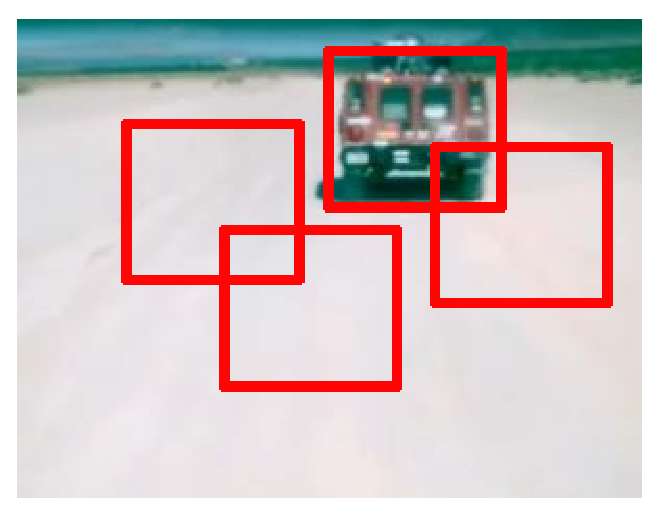
\includegraphics[width=.5\columnwidth]{images/figure2a.eps}}
  \subfloat[]{\label{subfig:(b)} 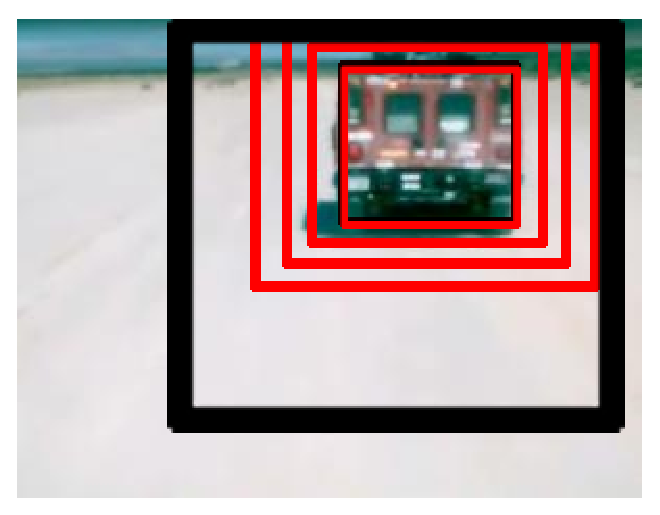
\includegraphics[width=.5\columnwidth]{images/figure2b.eps}}
  \caption{The red boxes show the analyzed regions and the black boxes represent the $WOS$. 
  (a) The regions are compared with a $ROI$ using the same scale. 
  (b) The regions are compared with a $ROI$ using different scales.}
  \label{fig:multires}
\end{figure}

The Algorithm \ref{alg:multires} describes the method explicated in the 
Fig. \ref{fig:multires}(b), It is represented by the function 
$multiscale\_match\_criterion()$ and It is used in the Algorithm \ref{alg:system}.

\begin{algorithm}
 \KwData{A $ROI$, your position $P_0$ and an image frame $I_i$. }
 \KwResult{The best matched analysis region, $AR$, your position 
 $P_{max}$ and the correlation value,$r_{max}$, with the $ROI$. }
 ~\\
 $W$: Width of $ROI$\;
 $H$: Height of $ROI$\;
 $L$: Search arm in pixels (defined by the user)\;
 $\alpha \leftarrow 0.8$\;
 $r_{max} \leftarrow -1.0$\;
 ~\\
    \While{$0.8 \leq \alpha \leq 1.4 $}{
      
      $A \leftarrow get\_corr\_matrix(ROI,P_0,\alpha,L,I_i)$\;

      $p_i$: position $(x_i,y_i)$ of maximum value in $A$\;

      $r \leftarrow A(p_i)$\;

      \If{$r > r_{max}$}{
	$r_{max} \leftarrow r$\;
	$P_{max} \leftarrow P_0 +p_i-(L,L)$\;
	$\alpha_{max} \leftarrow \alpha$\;
      }
      ~\\
      $\alpha \leftarrow \alpha +0.05$\;
    }
    
$AR$: Region in $I_i$, at point $P_{max}$, with size $\alpha W$ by $\alpha H$\;      
\Return $\{AR,P_{max},r_{max}\}$\;
~\\
\caption{$multiscale\_match\_criterion(ROI,P_0,I_i)$ function.}
\label{alg:multires}
\end{algorithm}

We can see that the Algorithm \ref{alg:multires} uses internally
the function $get\_corr\_matrix()$, this function returns a matrix 
with the correlation values of $ROI$ with the analyses of regions
inside the $WOS$ around the central point $P_0$. 
All the procedure of this function can be seen detailed in the Algorithm \ref{alg:multires2}.

\begin{algorithm}
 \KwData{A $ROI$, your position $P_0$, a departure factor $\alpha$, the search arm 
 $L$ and an image frame $I_i$. }
 \KwResult{The correlation matrix $A$, compound around the point $P_0$ of $I_i$. }
 ~\\
 $W$: Width of $ROI$\;
 $H$: Height of $ROI$\;
 $lin_0$: The first term of $P_0$\;
 $col_0$: The second term of $P_0$\;
 $A$: Creates a square matrix of $2L+1$ pixels by side and fill it with zeros\;

 ~\\
    \For{$-L \leq lin \leq L$}{
    \For{$-L \leq col \leq L$}{
      $AR$: Region in $I_i$, at point $(lin_0+lin,col_0+col)$, with size $\alpha W$ by $\alpha H$\;
      $AR \leftarrow $ rescale $AR$ to $ROI$ size\;
      
      $Q$ is filled according the Eq. (\ref{eq:Q})\;
      $A(L+lin,L+col) \leftarrow CCP(Q\times ROI,Q\times AR)$\;

    }
    }
    
\Return $A$\;
~\\
\caption{$get\_corr\_matrix(ROI,P_0,\alpha,L,I_i)$ function.}
\label{alg:multires2}
\end{algorithm}


%onde estava, onde esta agora
%que tamanho tinha que tamanho tem.

\end{comment}

%%%%%%%%%%%%%%%%%%%%%%%%%%%%%%%%%%%%%%%%%%%%%%%%%portugues%%%%%%%%%%%%%%%%%%%%%%%%%%%%%%%%%%%%%%%%%%%%%%%%%%

\subsection{Critério de busca em camadas}

O critério de busca do objeto de interesse está baseada na técnica $PIV$; 
consequentemente, é necessário definir alguns parâmetros para executar  
este algoritmo. Assim nos temos, a região de interesse ou $ROI$ 
 que é a região ou porção da imagem que contém
o objeto de interesse, também precisamos uma janela de busca ou $WOS$
que é a região onde serão analisadas regiões para identificar a $ROI$. 
Na técnica $PIV$ tradicional, quando é analisada uma imagen, 
a posição do objeto de interesse na imagem é obtida a partir 
da posição da região analises na imagem com o valor de $CCP$ mais próximo de $1.0$,
quando comparada com a $ROI$. 
Essa análise consiste na divisão da $WOS$ em regiões de analises que sejam do tamanho da $ROI$, pois o $CCP$
compara imagens do mesmo tamanho.

A Figura \ref{fig:multires}(a) mostra a aplicação da técnica $PIV$ (tradicional)
para duas dimensões, onde as regiões de analises na $WOS$
são comparadas com a $ROI$. 
A Figura \ref{fig:multires}(b) representa uma aplicação em 3 dimensões da técnica $PIV$. 
Neste ponto, inclui-se camadas, estas consistem na diminuição e aumento da regiões de analises os quais 
contemplam casos de afastamento e aproximação do objeto, respectivamente.

\begin{figure}[H]
\centering
  \subfloat[]{\label{subfig:(a)} 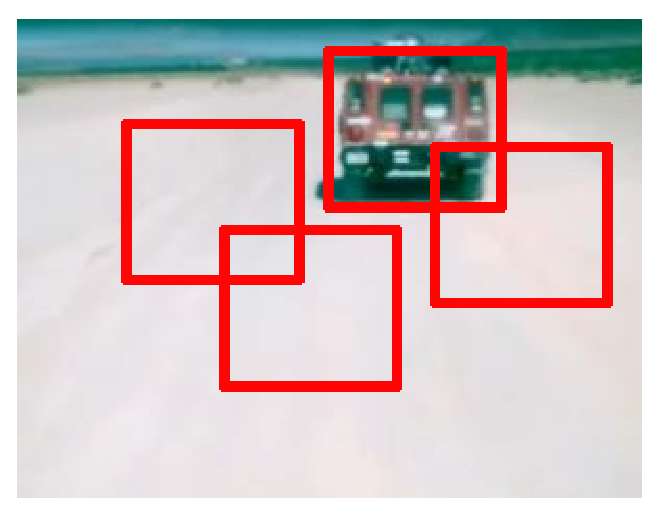
\includegraphics[width=.5\columnwidth]{images/figure2a.eps}}
  \subfloat[]{\label{subfig:(b)} 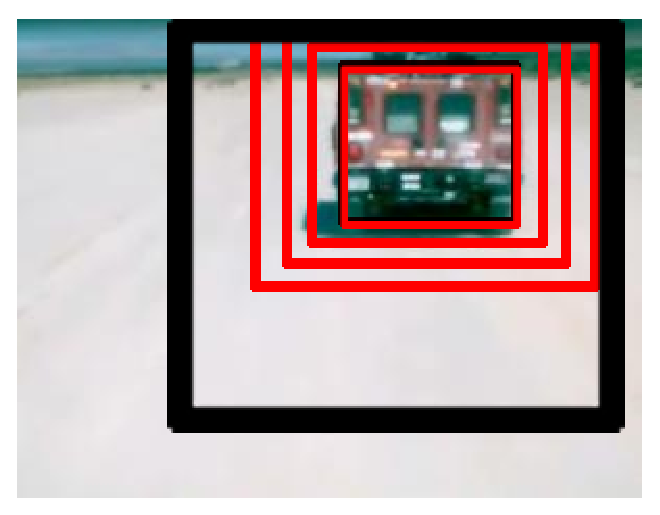
\includegraphics[width=.5\columnwidth]{images/figure2b.eps}}
  \caption{Os retângulos vermelhos mostram as regiões analisadas e o retângulo preto representa a $WOS$. 
  (a) As regiões de analises da $WOS$ são comparadas com a $ROI$ em uma única camada. 
  (b) As regiões de analises da $WOS$ são comparadas com a $ROI$ em diferentes escalas é dizer múltiplas camadas.}
  \label{fig:multires}
\end{figure}

O algoritmo \ref{alg:multires} descreve o método usado na Figura \ref{fig:multires}(b), o qual
está representado pela função $multiscale\_match\_criterion()$ no algoritmo \ref{alg:system}.
\begin{algorithm}
 \KwData{ $ROI$, posição $P_{i-1}$ do objeto de interesse na imagem $I_{i-1}$ e a imagem $I_i$. }
 \KwResult{A região $AR$ com a mais alta correlação, a posição 
 $P_{max}$ e o valor $r_{max}$ da correlação com a $ROI$. }
 ~\\
 $W$: Width of $ROI$\;
 $H$: Height of $ROI$\;
 $L$: Search arm in pixels (defined by the user)\;
 $\alpha \leftarrow 0.8$\;
 $r_{max} \leftarrow -1.0$\;
 ~\\
    \While{$0.8 \leq \alpha \leq 1.4 $}{
      
      $A \leftarrow get\_corr\_matrix(ROI,P_{i-1},\alpha,L,I_i)$\;

      $p_i$: position $(x_i,y_i)$ of maximum value in $A$\;

      $r \leftarrow A(p_i)$\;

      \If{$r > r_{max}$}{
	$r_{max} \leftarrow r$\;
	$P_{max} \leftarrow P_{ROI} +p_i-(L,L)$\;
	$\alpha_{max} \leftarrow \alpha$\;
      }
      ~\\
      $\alpha \leftarrow \alpha +0.05$\;
    }
    
$AR$: Region in $I_i$, at point $P_{max}$, with size $\alpha_{max} W$ by $\alpha_{max} H$\;      
\Return $\{AR,P_{max},r_{max}\}$\;
~\\
\caption{$multiscale\_match\_criterion(ROI,P_{i-1},I_i)$ function.}
\label{alg:multires}
\end{algorithm}
O algoritmo \ref{alg:multires} usa internamente a função $get\_corr\_matrix()$,
esta função tem como saída uma matriz com os valores da correlação da $ROI$ e as regiões de analises na $WOS$
em torno ao ponto $P_{i-1}$. Todos os processos da função $get\_corr\_matrix()$ são detalhados no algoritmo
\ref{alg:multires2},
\begin{algorithm}
 \KwData{$ROI$, posição $P_{i-1}$ sendo este o centro da $WOS$, 
 fator de aproximação $\alpha$ relativa à distancia $d_{ROI}$, braço de busca 
 $L$ e a imagem $I_i$. }
 \KwResult{A matriz de correlação $A$, da regiões ao redor do ponto $P_{i-1}$ da imagem $I_i$. }
 ~\\
 $W$: Width of $ROI$\;
 $H$: Height of $ROI$\;
 $lin_c$: The first term of $P_{i-1}$\;
 $col_c$: The second term of $P_{i-1}$\;
 $A$: Creates a square matrix of $2L+1$ pixels by side and fill it with zeros\;

 ~\\
    \For{$-L \leq lin \leq L$}{
    \For{$-L \leq col \leq L$}{
      $AR$: Region in $I_i$, at point $(lin_c+lin,col_c+col)$, with size $\alpha W$ by $\alpha H$\;
      $AR \leftarrow $ rescale $AR$ to $ROI$ size\;
      
      $Q$ is filled according the Eq. (\ref{eq:Q})\;
      $A(L+lin,L+col) \leftarrow CCP(Q\times ROI,Q\times AR)$\;

    }
    }
    
\Return $A$\;
~\\
\caption{$get\_corr\_matrix(ROI,P_{i-1},\alpha,L,I_i)$ function.}
\label{alg:multires2}
\end{algorithm}
